% !TEX TS-program = pdflatex
\documentclass[10pt,twocolumn]{article} 

% required packages for Oxy Comps style
\usepackage{oxycomps} % the main oxycomps style file
\usepackage{times} % use Times as the default font
\usepackage[style=numeric,sorting=nyt]{biblatex} % format the bibliography nicely 

\usepackage{amsfonts} % provides many math symbols/fonts
\usepackage{listings} % provides the lstlisting environment
\usepackage{amssymb} % provides many math symbols/fonts
\usepackage{graphicx} % allows insertion of grpahics
\usepackage{hyperref} % creates links within the page and to URLs
\usepackage{url} % formats URLs properly
\usepackage{verbatim} % provides the comment environment
\usepackage{xpatch} % used to patch \textcite

\graphicspath{ {./images/} }
\bibliography{refs.bib}
\DeclareNameAlias{default}{last-first}

\xpatchbibmacro{textcite}
  {\printnames{labelname}}
  {\printnames{labelname} (\printfield{year})}
  {}
  {}

\pdfinfo{
    /Title (Image Search In Video Platforms With The Fuzzy C-Means Algorithm)
    /Author (Christopher Linscott)
}

\title{Image Search In Video Platforms With The Fuzzy C-Means Algorithm}

\author{Christopher Linscott}
\affiliation{Occidental College}
\email{clinscott@oxy.edu}

\begin{document}

\maketitle

% Refer to rubic: https://docs.google.com/document/d/1oiXngqxh30ADXVPfOEnNuBNX1DGFmmExI6DoGZNdrs0/edit

\section{Problem Context}

Often, when learning new topics or exploring new areas, one may come across a topic or object they’ve never seen before. Getting more information feels paradoxical, as obtaining further knowledge given only visual context is difficult; in a sense, you “don’t know what you don’t know”. In general, current video recommendation methods rely on textual information about the video using keywords \cite{Stanford2021}. Without knowing the name or a related keyword, one cannot simply search the web in hopes for an answer. Not only does image search help users tell the search engine what they’re looking for (without ambiguity), but image-related search removes the need to annotate images online with keywords as image similarity can be used as a heuristic \cite{Adrakatti2016}.

The solution I propose involves utilizing video platforms like YouTube, as a means to solve this information gap using related videos, while also offering times within videos where the relevant content is found. A user would insert an image of an object in real life or even a drawing (from their lecture notes for example), and my project would return videos with related images either in the thumbnail or the video frames. If related video frames are found within the video, times corresponding to these frames will additionally be returned.

YouTube videos can be broken down into images through both the thumbnail, an image preview of the video content, and the individual frames which make up the same video. With my project, we essentially create "baskets" of videos which relate to each other by visual characteristics (called “features”). Upon inserting an image, finding relevant information means finding the basket of images (that refer to videos or video frames) which relate to our input image by comparing features. By utilizing video frames as opposed to simply other images (like thumbnails), my project speeds up the searching process by returning a time within the video. From an educational perspective, not only does this help students fulfill these information gaps through videos, but it can speed up the studying process as users don’t always have to sift through a video to grab the relevant information.

\section{Technical Background} 

Creating baskets of related images and video frames requires using clustering (an unsupervised version of classification). To be more specific, clustering is the “method of segmenting a population into subgroups where members are more similar to each other than to members of other subgroups based on certain observed features” \cite{C3Clustering}. To be kurt, clustering is the methodology of creating subgroups of videos which relate to each other based on characteristics of one another. It’s referenced as unsupervised as the images and video frames we give will not have any pre-existing labels on them; finding datasets large enough, which includes these labels or categories, is a hard task in itself. Our population here will be a collection of images corresponding to objects in the real world, drawings, YouTube thumbnails, and YouTube video frames. Features, in this context, are visual characteristics of these images that may relate to other images.

Fuzzy clustering, a type of clustering, says that a data point (i.e. an image) always resides uniquely inside a cluster (i.e. basket), but that it can reside in more than one cluster based on varying amounts of “belonging” \cite{PrasadClustering}. Each image would have a belongingness metric of some value between 0 and 1 to some number of clusters; you may also see this referenced as a “membership” metric. As images may have multiple components (including text, a background, people, and objects), this is more viable as opposed to a more strict clustering algorithm such as hierarchical clustering (where the baskets may be too small). Similar to k-means clustering, the number of clusters must be specified. For our use case, the specification of our clusters is normal, as we want to know how big or small these “baskets” may end up. Unlike k-means clustering, fuzzy clustering is preferred for images with lots of overlapping \cite{PrasadClustering}, which is exactly what should occur with these different types of images, as the images have related objects, shapes, and backgrounds.

The algorithm used to perform Fuzzy clustering for this project will be the Fuzzy C-Means algorithm, which utilizes this function:

For a datapoint(image) I, the given total sum of distances between all k clusters, in relation to a datapoint's belongingness value (for each cluster) with them
can be calculated as followed:

\[ I(k, m)  =  \sum_{j=1}^{k} \sum_{x_i \in C_j} u_{ij}^{m}(x_i - u_j)^2 \]

where \(u_{ij}\) is the degree of belongingness of a data point \(x_i \) to a cluster \(C_j \) which is between 0 and 1, \(u_j \) is the center of the cluster, and \(m \) is the fuzzifier (which converts strict into “fuzzy” sets with more blurred lines) \cite{PrasadClustering}. This function uses Euclidean distance, which is why \((x_i - u_j)^2 \) is present. The function takes in two parameters: \(k\), which represents the number of clusters and \(m \), the fuzzifier, which can be adjusted to make stricter or fuzzier clusters. The Fuzzy C-Means algorithm seeks to minimize this function, which minimizes the Euclidean distance between a given data point and the centers of all the clusters. By utilizing membership values, the algorithm places importance on clusters to be closer or farther from a data point depending on the value of belongingness for that datapoint; if a datapoint belongs greatly to a cluster, the cluster should be much closer to it (and vice versa). By minimizing the distance metric between a cluster’s center and its neighboring related (belonging) data points, it makes baskets of datapoints (or images) which relate to each other visually, given that the computation of an image's visual characteristics fairly represents its features. It should be noted that we have freedom in how strict it makes these clusters, as a large \(m \) suppresses outliers in datasets, as the higher values of \(m \) allows more objects per cluster (i.e. sharing between clusters) \cite{Schwammle2010}. Whereas, with lower values, we allow less cluster “sharing” (i.e. less images to be partial members in many clusters). To determine the initial centroid (or initial place acting as the center of the cluster) as well as the membership values (overtime) we can solve for the following equations as done in Schwammle’s paper: 
\[u_j = \frac{\sum_{i=1}^N u_{ij}^m x_i}{\sum_{i=1}^Nu_{ij}^m}\] 

\[u_ij = \frac{1}{\sum_{s=1}^k \frac{(x_i - u_j)^2}{(x_i - u_s)^2} }\] 

The first equation calculates the positions of the centroids, by effectively taking the mean of the positions of its most related datapoints; datapoints with a higher belongingness will have a larger effect on the cluster's position (as \(u_{ij}\) approaches 1). To take the average of this, it divides by the same belongingness metric of all the points.
The second equation calculates the new membership values of the datapoints, by calculating the Euclidean distance of the datapoint i to cluster j, and dividing it by the sum of the distances between all the other k-1 clusters. If a datapoint is much closer to a given cluster, the distance to the other clusters will be much larger; by taking the reciprocal of this division, we get the correct belongingness metric to the cluster. By utilizing these equations, we can determine what clusters an image resides in (and how much it belongs to a given cluster), and recalculate the relative “baskets”. However, we have no way to get the initial data points.

However, the main input for a clustering algorithm is datapoints, which have some dimension d. Inserting a 2D image simply means inserting \( h * w * 3\) pixels where \(h\) is height, \(w\) is width, and 3 represents the three channels of color (red, green, blue) for a given image. While this will be iterated in Methods, pixels are not a good approach to clustering images as they do not derive meaningful clusters (refer to Methods).

In order to determine information about an image, in processing images and assigning them a belongingness metric, we need to take into account the objects, edges, shapes, and other characteristic of objects that may render useful. To do so, we can utilize a convolutional neural network (CNN). By doing so, we can retrieve an "activation" or how much of a particular feature is in a given image. Thereby, we can determine the activation of surroundings, noise, objects, and people in a given image. By assessing these visual characteristics, we can derive a datapoint for a particular image, and utilize the function and algorithms previously discussed.
By utilizing these activations, we can either flatten them and insert them as one single datapoint of dimension d, or take inspiration from Kavitha’s fuzzy algorithm, utilized for the classification of satellite images, as follows: F is a satellite image, NB is the natural background, MM includes man-made objects, and NO describes noises \cite{Kavitha2020}.
\[F(i, j) = NB(i,j) + \sum_{x=1}^{n} MM(i, j) + NO(i, j) \]

By repurposing this equation to account for an input image (or image in the dataset) to include objects and people, we can effectively begin to determine the data points for a given image. Utilizing this equation referenced above, we can utilize the Fuzzy C-Means algorithm as a means to cluster and determine how strongly a given image belongs to a given number of clusters.

\section{Prior Work}

Many image-related applications have been developed around gathering information. A popular application which has come out is Google Lens, an application which in real time can analyze an image (whether it has text or a given object) and identify the object or text. Furthermore, image-related search applications, such as Google’s reverse image search, are very useful in determining the source of an image or determining similar images based on an input image. In fact, it’s being used often for educational purposes such as with plant identification \cite{Moore2018}. In a similar way to how Google Lens and Google’s reverse image search aims to solve the information gap (given only visual context), my application serves to solve it using related videos as opposed to a purely trained AI model on the classification of objects. \\ 
\indent To go on, researchers at Stanford have utilized video frames within a given video (along with labeled good and bad thumbnails) to train a convolutional neural network to determine what frames of that video would constitute as a good “thumbnail”, or image preview to capture a user’s attention \cite{Stanford2017}. Extending this idea, we can utilize the video frames in order to gather images to act as “markers” for the videos; when an user-given image matches, it references the video and/or the time within it.\\
\indent Along with classifying YouTube thumbnails together, neural networks have also proven to be able to learn to cluster YouTube thumbnails together, categorizing them into different categories without the help of tags (i.e. labeled categories on the videos). Utilizing k-means clustering, they were able to compare and determine that a clustering algorithm could categorize videos by their thumbnails as well as YouTube did manually with tags \cite{Stanford2021}. So, with this paper in mind, as opposed to using classification like the first group of Stanford researchers, my project shifted toward using clustering because my datasets are not labeled and labeling data is very tedious. \\
\indent However, there are many ways (or algorithms) to cluster a dataset, depending on the type of data one is handling. Therefore, analyzing papers which tackled a similar problem led me to Kavitha’s paper, which retrieves images that are relevant to the user given image, for the purposes of getting information that’s useful for natural disaster management. The paper pushes that other image-retrieval algorithms are incomponent in terms of efficiency with clustering images, and that utilizing the Fuzzy characteristic algorithm can achieve great precision with better efficiency \cite{Kavitha2020}. Furthermore, an article about the many methods/algorithms of clustering agreed that Fuzzy algorithms are best for image segmentation which aligns with the arguments of the paper \cite{PrasadClustering}. As my project will involve deriving related images and image segmentation (in order to make the images more meaningful), my project landed on the Fuzzy C-Means Algorithm (as opposed to a K-means clustering) as the resource for clustering my images all together and creating these baskets.

\section {Methods}

From a high level standpoint, the approach involves taking an input image, running it through a convolutional neural network (CNN), grabbing the corresponding features derived from the CNN, and utilizing these as data points for the clustering algorithm, Fuzzy C Means (FCM). The clustering algorithm will take these data points and create baskets of videos based on similar features, thereby creating clusters of related videos which are similar to each other by visual characteristics. 

Clustering by the features of the convolutional neural network will result in much less noise and more meaningful generated “classes” or categories of the image clusters. If the raw images are small enough, we may be able to do clustering utilizing the individual pixels. However, possible noises present in image and video manipulation may interfere too heavily with this type of clustering, especially if the wrong value of “fuzziness” is chosen, having higher noise interference \cite{Zhang2019}. As well as, the number of features extracted by individual pixels may be far too many to be meaningful or considerable. As an example, applying K-Means clustering to raw image data of colored images, showed the strengths of the algorithm when the objects and colors were alone and distinct (Figure 1). However, when the image had objects of similar colors interleaved (Figure 2), the clustering algorithm struggled much more. Therefore, in the context of image manipulation and colored images, a convolutional neural network can help derive features from images such as edges, shape, position, distribution of colors, and edge orientation \cite{Lavrenko2014}.

\begin{figure}[h]
 \centering
 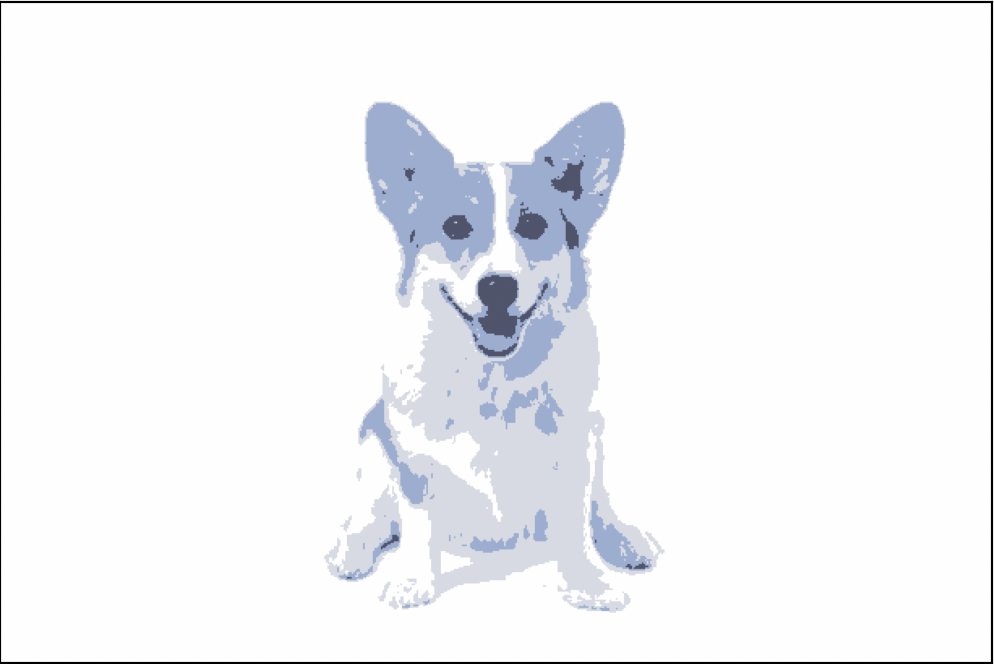
\includegraphics[scale=0.2]{corgi-white.png}
 \vspace{20px}
 \caption{The K-Means clustering algorithm (f=2 for Fuzzy C Means) applied to an image of a Corgi in a white back-ground.}
 \label{corgi:white}
\end{figure}

\begin{figure}[h]
 \centering
 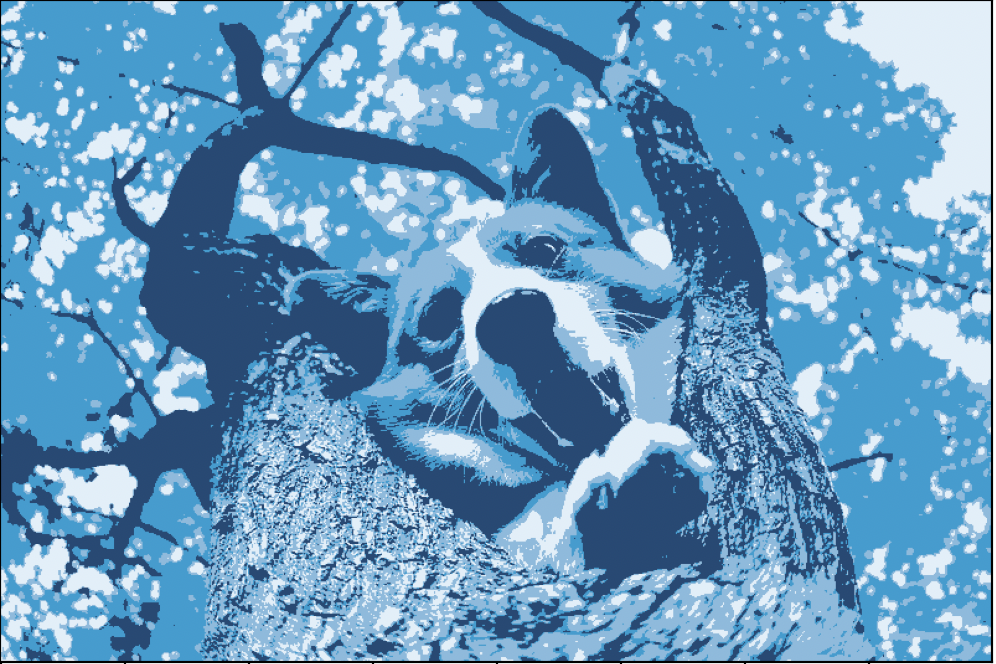
\includegraphics[scale=0.2]{corgi-tree.png}
 \vspace{20px}
 \caption{The same clustering algorithm applied to an image of a corgi on a tree. Note how pixels (i.e. colors) of the tree and Corgi get grouped together.}
 \label{corgi:tree}
\end{figure}


With this in mind, I plan to utilize a CNN that takes an input image of a given height, width, and three channels (\(Red, Green, Blue\)) and returns features \( {f1, \cdots, fn} \) which will act as data points of dimension \(n \) for the Fuzzy C Means Algorithm. The convolutional neural network will have several convolutional layers which have 3 individual kernels/filters underneath (for each of the different color channels red, green, and blue). These kernels will be represented by a 3x3 matrix of either set values (Sobel filters), randomly initialized, or zero initialized values. My plan is the outer layers will have more set values (such as filters for horizontal or vertical edges), and the inner layers will have more randomly initialized or zero initialized values. The 2-D matrices will be mapped over the image by computing a given value for a given set of 9 (3x3) pixels for one channel (R, G, or B); computing this value will requiring the cross product or summing up all the multiplications of overlapping values of pixels and the filter together. The values generated by this multiplication will represent the activation (i.e. if it detects a given feature, such as an edge). However, an activation of 40 versus -10 can be seen as ambiguous and meaningless in terms of a single neuron (where we only care if it fires). 

Upon the outputs of the kernels (called a feature map), they will be inserted into a ReLU activation function, which computes the activation (i.e. if the feature is recognized) based on if the value is positive (activates) or negative (doesn’t activate). After this convolutional layer and input through the ReLU function, the values are now simply activations or non activations. The final important layer of this convolutional neural network will be the max pooling layer, which in short allows for “translational invariance”, or the idea that if the image is rotated, sized differently, or viewed in different lighting \cite{Khandelwal2018}, that the object will still be recognized; this is necessary in the previously stated context of image manipulation. The max pooling layers will summarize the statistics of nearby locations, by also utilizing a filter of size 2x2 or 3x3. In short, the pooling layer will take the input from the previous layer and condense by selectively looking at a grid of pixels (the same size as the filter) and grabbing the maximum value of those pixels as its output. So, for a 2x2 filter, the pooling layer will take 4 pixels and condense into one pixel which has the maximum activation of that individual pixel; this reduces the size of the output and “pools” activations together. By reducing the size of input entering the next layer, it reduces the computational load, and by using max pooling (or grabbing the highest values only), it highlights the parts of the feature which most align with the given feature the filter is trying to extract. As well as, by max pooling, this reduces overfitting (since we only look at general features by condensing rather than at outliers). The idea with all of these layers is to create virtually many “feature” detectors which can derive features while reducing computational complexity, noise, and overfitting. 

With these layers in mind, the convolutional neural networks will have these convolutional and pooling layers interleaved, so that the convolutional layer uses convolution to find the filter and the pooling layer uses pooling to effectively “highlight” the activation it finds and reduce the size of the input image before it reaches the inner layers (where often you’ll be looking at smaller parts of an image). The output of this final convolutional neural network will be a three-dimensional matrix of pooled values representing varying amounts of activation \cite{Arc2018}; to convert this into a datapoint, the matrix will be flatten into a single vector (i.e. one dimension). Normally, there would be a final layer, called the Fully Connected Layer (FC), which can be utilized to identify the object. However, given I want to simply cluster by similar objects and not identify them, omitting this final layer and placing the flatten vector into my clustering algorithm (FCM) is my preferred method. Fuzzy C-Means and K-Means are both computationally efficient at O(n) and O(knt) respectively \cite{Mittal2021}, and therefore utilizing either can save on computational costs, especially with the high number of pixels and features. 

Given the features from the CNN as an array of features \(f_{1} \cdots f_{n}\), the Fuzzy C-Means algorithm will look at these as a singular datapoint of dimension (or size) n. The main idea behind the FCM algorithm is given all the data points and a fuzzifier (a number denoting how hard or soft the clustering is), to compute suitable centers of groups of videos/video frames based on a common feature or group of features that are similar between them. The output will be the positions of the centers of the centroids, and a corresponding table of the images and their corresponding clusters denoted by a number j. To compute these centers, we’ll use the Fuzzy C-Means algorithm with the following pseudocode.

% \begin{algorithmic}
%   \begin{algorithm}
%     \State $f \gets $4
%   \end{algorithm}
	
	% \State $data_points \gets [f_1, f_2, …, f_n]
	% \State $centroids \gets [[0.1, 0.4, …, 0.05], …, k] 
	% \State $diff \gets $1
	% \While diff:
	% Calculate new centroid positions based on membership values of data_points
	% Recalculate the new membership values based on these new centroid positions compared to old ones
	% Calculate diff to be the difference between the original centroid position and new centroid position
	% If the diff is large enough, break
	
	% (Optional) Decide on a primary cluster for each datapoint depending on the largest membership it has
	
	% \Returns centroid positions, datapoint and corresponding clusters
% \end{algorithmic}

After these clusters have been computed, now the algorithm is set and ready to be tested. Placing a given image through the CNN gives us a relevant datapoint. Using this datapoint, we can determine initially what basket to check (by the Euclidean distance metric), as well as other viable options in order of membership value. Based on the data points distance to other data points, these corresponding images and video IDs will be returned first (since they are most similar in terms of visual characteristics). The progression of “relevance” will be determined by if the primary clusters are the same or not and then the corresponding distance to that datapoint. By computing this, we’ll get a list of videoIDs and their corresponding relevance depending on these factors. 

\section{Evaluation}

Not only does the evaluation of clustering algorithms allow us to test the cluster for the features/classes it groups upon, but it allows the developer (or myself) to identify and eliminate outliers, compare to human judgments, and understand the makeup of the data itself \cite{Lavrenko2014}. Within the context of this COMPS Project, evaluating the strengths and weaknesses of Fuzzy C-Means and K-Means clustering algorithms allowed me to introduce the idea of utilizing a convolution neural network.

To evaluate an image segmentation algorithm, it requires that we assess the strength of the clustering algorithm based on the meaningful classes that it generates. In other words, it should have clusters (even if they’re unlabeled), that resemble characteristics or blobs of image data that a human may draw out as meaningful. In our previous example, the Corgi in the tree, while clustered, was clustered into several different parts compared to just the Corgi in the white background. It’s clear that pixels do not serve as an identification for features, as colors can be shared by different parts or different objects within the image (in this case, the Corgi and the tree). There are mainly two parts I propose to evaluate a given clustering algorithm: the strength of these clusters (i.e. how well can it cluster pixels of an object together in comparison to a human) and how relevant are the videos to each other.

If we want to evaluate the strength of these clusters, there are several methods, but I propose utilizing combinations of comparisons between the prediction and ground truth such as Intersection-over-Union and a Confusion Matrix as these are not only widely used representations (making them easy for others to evaluate themselves based on the results) \cite{Mittal2021}, but they are not mathematically difficult to represent nor compute. Not to mention, it’s very easy to compare as we’re simply comparing pixel-to-pixel for clusters (as we’ll know all the pixels and their clusters given our methods) as opposed to instance segmentation which requires identifying the objects/classes.

A confusion matrix consists of representing the accuracy, precision, and recall based on storing the true values (true positive/negative) and negative values (false positive/negative) in a 2x2 matrix \cite{Jordan2018}. By utilizing formulas for accuracy, precision, and recall, we can define how accurate versus precise our clustering may be in relation to human judgment \cite{Jordan2018}. Rather than having to ask human judges to define the accuracy or even the cluster for us, we can determine how well it predicts the ground truth in comparison to previously human-segmented images. In turn, our evaluation can determine how strong the clustering algorithm can group similar features (and therefore similar videos) together without having to ask for human judgment.

While the clustering algorithm may be solid for determining images of related visual similarity, the last question to ask is whether these clustering algorithms lead to related videos (of most importantly related content). As computers cannot evaluate the similarity between videos based on content, my plan is to ask others to test the program with test images of their own (and my own) and determine whether the related videos are helpful or not. As the primary user may be a student or researcher, I may ask for related lecture notes, diagrams, and drawings with the intent of assessing the relevance of the videos my program generates. While this may be qualitative, a quantitative judgment such as those in the previous paragraph, may not be able to measure helpfulness due to a disparity between the video image similarity and the video content similarity.


\printbibliography


\end{document}
